%; whizzy document -ps gv
% latex beamer presentation.
% platex, latex-beamer でコンパイルすることを想定。 

%     Tokyo Debian Meeting resources
%     Copyright (C) 2007 Junichi Uekawa

%     This program is free software; you can redistribute it and/or modify
%     it under the terms of the GNU General Public License as published by
%     the Free Software Foundation; either version 2 of the License, or
%     (at your option) any later version.

%     This program is distributed in the hope that it will be useful,
%     but WITHOUT ANY WARRANTY; without even the implied warranty of
%     MERCHANTABILITY or FITNESS FOR A PARTICULAR PURPOSE.  See the
%     GNU General Public License for more details.

%     You should have received a copy of the GNU General Public License
%     along with this program; if not, write to the Free Software
%     Foundation, Inc., 51 Franklin St, Fifth Floor, Boston, MA  02110-1301 USA

% 実行順番
% sudo  ~/bin/usb-macbook-ir.c &
% real presentation (shell-command (concat "DISPLAY=:0.1 xpdf -fullscreen " (replace-regexp-in-string "tex$" "pdf"(buffer-file-name)) "&"))
% DISPLAY=:0.1 xpdf -fullscreen 

\documentclass[cjk,dvipdfmx,12pt]{beamer}
\usetheme{Tokyo}

%  preview (shell-command (concat "xpdf " (replace-regexp-in-string "tex$" "pdf"(buffer-file-name)) "&"))
%  presentation (shell-command (concat "xpdf -fullscreen " (replace-regexp-in-string "tex$" "pdf"(buffer-file-name)) "&"))

%http://www.naney.org/diki/dk/hyperref.html
%日本語EUC系環境の時
\AtBeginDvi{\special{pdf:tounicode EUC-UCS2}}
%シフトJIS系環境の時
%\AtBeginDvi{\special{pdf:tounicode 90ms-RKSJ-UCS2}}

\title{東京エリア Debian 勉強会}
\subtitle{資料}
\author{上川 純一 dancer@debian.org\\IRC nick: dancerj}
\date{2007年5月19日}
\logo{
\includegraphics[width=8cm]{image200607/openlogo-light.eps}}


% 三択問題用
\newcounter{santakucounter}
\newcommand{\santaku}[5]{%
\addtocounter{santakucounter}{1}
\frame{\frametitle{問題\arabic{santakucounter}. #1}
%問題\arabic{santakucounter}. #1
\begin{minipage}[t]{0.8\hsize}
 \begin{itemize}
 \item
      \begin{minipage}{0.2\hsize}
      
\includegraphics[width=0.9\hsize]{image200703/janken-A.png}\end{minipage} 
       \begin{minipage}{0.6\hsize}
       A #2\end{minipage}\\
 \item
      \begin{minipage}{0.2\hsize}
      
\includegraphics[width=0.9\hsize]{image200703/janken-B.png}\end{minipage} 
       \begin{minipage}{0.6\hsize}
       B #3\end{minipage}\\
 \item
      \begin{minipage}{0.2\hsize}
      
\includegraphics[width=0.9\hsize]{image200703/janken-C.png}\end{minipage} 
       \begin{minipage}{0.6\hsize}
       C #4\end{minipage}\\
 \end{itemize}
\end{minipage}
}
\frame{\frametitle{問題\arabic{santakucounter}. #1}
%問題\arabic{santakucounter}. #1
\begin{minipage}[t]{0.8\hsize}
\begin{itemize}
 \item
      \begin{minipage}{0.2\hsize}
      
\includegraphics[width=0.9\hsize]{image200703/janken-A.png}\end{minipage} 
       \begin{minipage}{0.6\hsize}
       A #2\end{minipage}\\
 \item
      \begin{minipage}{0.2\hsize}
      
\includegraphics[width=0.9\hsize]{image200703/janken-B.png}\end{minipage} 
       \begin{minipage}{0.6\hsize}
       B #3\end{minipage}\\
 \item
      \begin{minipage}{0.2\hsize}
      
\includegraphics[width=0.9\hsize]{image200703/janken-C.png}\end{minipage} 
       \begin{minipage}{0.6\hsize}
       C #4\end{minipage}\\
\end{itemize}
\end{minipage}
\begin{minipage}[t]{0.15\hsize}
答えは:

\vspace{1cm}

  {\huge \hspace{1cm}#5}
  \hspace{-6cm}\includegraphics[width=4cm]{image200703/janken-#5.png}
 \end{minipage}}
}

\begin{document}
\frame{\titlepage{}}

\section{Intro}

\begin{frame}
 \frametitle{本日のagenda}
\begin{minipage}[t]{0.45\hsize}
  \begin{itemize}
  \item 注意事項
	\begin{itemize}
	 \item 飲食禁止
	 \item 政治/宗教/営利活動禁止
	\end{itemize}
  \item quiz
  \item Debconf7 リハーサル
	\begin{itemize}
	 \item pbuilder 
	 \item superh
	\end{itemize}
 \end{itemize}
\end{minipage} 
\begin{minipage}[t]{0.45\hsize}
 \begin{itemize}
  \item エッチ
	\begin{itemize}
	 \item サーバをエッチにしてみました
	 \item 事前課題紹介
	 \item エッチワークショップ
	\end{itemize}  
\item Debian 勉強会の今後の企画の検討
 \end{itemize}
\end{minipage}
\end{frame}

\section{最近}

\begin{frame}
 \frametitle{前回のagenda}
\begin{minipage}[t]{0.4\hsize}
  \begin{itemize}
  \item 注意事項
	\begin{itemize}
	 \item 飲食禁止
	 \item 政治/宗教/営利活動禁止
	\end{itemize}
  \item 最近事情 etchのリリースについて
  \item 事前課題紹介
  \item quiz
 \end{itemize}
\end{minipage} 
\begin{minipage}[t]{0.4\hsize}
 \begin{itemize}
  \item quilt 
  \item darcs 
  \item git
 \end{itemize}
\end{minipage}
\end{frame}


\begin{frame}{Debian 常識クイズ}

Debian の常識、もちろん知ってますよね?
しらないとはずかしいけどしらないとは言えないいろいろなこと、
Debian Weekly News をベースに確認してみましょう。

\end{frame}

\santaku
{3月12日 Alioth で新規に使えるようになったバージョンコントロールシステムはどれか}
{Mercurial}
{RCS}
{git}
{A}

\santaku
{Robert Milanが goodbye-microsoft 0.4.0 の機能として発表したのは何か}
{Ubuntu 対応}
{etch 対応}
{Windows Vista 対応}
{C}

\santaku
{Aurelien Jarno が kFreeBSD の新しいインストールCDを発表したが、対象アー
キテクチャは何か}
{i386}
{i386 amd64}
{ppc hppa arm}
{B}

\santaku
{teTeX と TeXLive で何がおきたか?}
{TeXLive はもう古いので teTeX でおきかえる}
{teTeX はもう古いので TeXLive でおきかえる}
{TeX のコンセプトが古いのでもう両方ともやめる}
{B}

\santaku
{Debian etch の CD/DVD イメージは何枚分あるか}
{666 枚の CD と 13 枚の DVD}
{292 枚の CD と 39 枚の DVD}
{1枚のDVDに全部おさまる}
{B}


\begin{frame}{Debconf2007}
Debian Project の開発者をあつめて技術的な内容を討議する年次のカンファレンス

 \begin{tabular}{|c|c|c|r|}
 \hline
 年 & 名前 & 場所 & 参加人数 \\
 \hline
 2000 & debconf 0 &フランス ボルドー & \\
 2001 & debconf 1 &フランス ボルドー & \\
 2002 & debconf 2 &カナダ トロント & 90名 \\
 2003 & debconf 3 &ノルウェー オスロ & 140名 \\
 2004 & debconf 4 &ブラジル ポルトアレグレ &  150名 \\
 2005 & debconf 5 &フィンランド ヘルシンキ & 200名 \\
 2006 & debconf 6 &メキシコ オアスタペック & 300名 \\
 2007 & debconf 7 &スコットランド エジンバラ & ?名 \\
 \hline
 \end{tabular}
\end{frame}
\begin{frame}{Debconf7 発表練習}
 発表予定なのでリハーサルをします
 \begin{itemize}
  \item pbuilder  上川
  \item superh  岩松
 \end{itemize}
\end{frame}

\begin{frame}{}

pbuilder 論 by 上川
\end{frame}

\begin{frame}{Who am I?}
\begin{itemize}
 \item Junichi Uekawa, dancer@debian.org
 \item Lives in Japan, Debian JP Project Leader for 2007
 \item Debian Developer since 2000
 \item Interests: Audio-processing related tools, and 
       Debian quality maintenance related tools,
       Japanese localization, shared library packaging, 
       and more recently, Debian/MacBook related.
\end{itemize}
 
\end{frame}

\begin{frame}[containsverbatim]{pbuilder の使いかた基本 0/2}
  \begin{verbatim}
 pbuilder create 
 pbuilder update
 pbuilder build *.dsc
 pdebuild 
 \end{verbatim}
\end{frame}

\begin{frame}{pbuilder の使いかた基本 1/2}
\begin{tabular}{|l|p{8em}|p{8em}|}
\hline
操作 & 操作頻度 & 意味 \\
\hline
create & 最初に base.tgz を作成するときに一度 & ベースファイルシステムの作成 \\
update & 一日二回 (unstable のアップデートに伴う) & ベースファイルシステ
 ムの更新 \\
build & パッケージビルドのたび & Debianパッケージを chroot 内部でビルド
 する \\
\hline
\end{tabular}
\end{frame}

\begin{frame}{pbuilder の使いかた基本 2/2}
\begin{minipage}{0.4\hsize}
パッケージのメンテナンスの流れ
\\
(上川の場合)
\end{minipage}
\begin{minipage}{0.5\hsize}
  \includegraphics[height=0.8\vsize]{image200705/develcycle.eps}
\end{minipage}
\end{frame}

\begin{frame}[containsverbatim]{開発体制}

alioth project: \url{http://alioth.debian.org/projects/pbuilder}

\begin{verbatim}
git-clone
  ssh://git.debian.org/git/pbuilder/pbuilder.git
\end{verbatim}
\end{frame}

\begin{frame}{pbuilder backend variations}
\begin{minipage}{0.5\hsize}
 Motivation
\begin{itemize}
 \item limitation in chroot segregation (process space, filesystem)
 \item COW filesystem optimization
\end{itemize}
\end{minipage}\begin{minipage}{0.4\hsize}
  \begin{itemize}
  \item LVM
  \item UML
  \item cowdancer
  \item qemu
 \end{itemize}
\end{minipage}
\end{frame}

\begin{frame}{further ideas}
 \begin{itemize}
  \item install testing
  \item package testing
 \end{itemize}
\end{frame}

\begin{frame}{related tools}
 \begin{itemize}
  \item schroot
  \item piuparts
  \item autodebtest
 \end{itemize}
\end{frame}

\begin{frame}{}
 質問ありますか?
\end{frame}

\begin{frame}{}
superh by 岩松さん
\end{frame}

\begin{frame}{etch 紹介}

\begin{itemize}
 \item サーバをエッチにしてみました by 小室 文
 \item 事前課題紹介
 \item ワークショップ
\end{itemize}
\end{frame}

\begin{frame}{etch リリース}
\begin{itemize}
 \item 4月8日 リリース
 \item 4月12日 宴会開催
 \item 5月1日ころ 日本語版リリースノート完成
 \item 5月19日 Debian 勉強会のテーマに!
\end{itemize}
\end{frame}

\begin{frame}{}
サーバをエッチにしてみました by 小室 文
\end{frame}

%% 事前課題開始

\begin{frame}

事前課題

「エッチになって困った事」

\end{frame}

% (query-replace "\\subsection" "\\end{frame}\\begin{frame}")

\begin{frame}{kinnekoさん}

Debian勉強会の宿題なので、ちと考えてみる。

なんだろう。実はあまり使っていないので、困っていなかったりする。
sources.listはだいぶ前からsargeに書き換える習慣だし。

\begin{itemize}
 
 \item VMwareのバージョンの古いのを使っているので、動かなくなりそうで移行できていないこと。

 \item 移行ノウハウがまだ十分に出揃っていない感じなので、さらでインストールする以外はまだ怖いな。

 \item β のときには、d-i試したり、GLANTANKでインストールしてみたり、ARM(XScale)での自動ビルドをやってみたり、LiveCDの
 MAKAIのベース変更テストしてみたりしたけど、リリースされてからのほうがまったくさわっていないかも。疲れたというか、飽きたというか。

\end{itemize}
\end{frame}
\begin{frame}{kinnekoさん}
\begin{itemize}
 \item パッケージ配布サイトの正当性を確認するようになったけど、キーの取り込み手順をもっと自動化してほしいかも。ついつい、ぶつぶつ言われても放置しちゃう。

 \item SHアーキテクチャでは、Etchベースで最新は海老原さんところと、岩松さんところかな。どっちも、どういう方向に進むのか外からあまり見えないところが難。それと、早くから進めていたkogiidenaさんとこが低調なのが気がかりです。

 \item ARMでは、やっぱりDMAまわりが遅いままなので、Debianではちょっと使い物にならないです。EABIへの対応も、はじまったばかりですし、ちょっとどうなることやら。

 \item udevやinitramfsに移行しきれていないので、勉強しなきゃなとか。

\end{itemize}
\end{frame}
\begin{frame}{kinnekoさん}
\begin{itemize}

 \item Etchってどんなキャラだったか思い浮かばないこと。あ、Etch A Sketchか。絵は自分で書けってことね。それもUIは結構不自由な感じで。

 \item 逆にapt-buildがSargeではうまく動かないのです。SHやARMでしか試してないですけど。Etchでは快調です。
\end{itemize}


\end{frame}\begin{frame}{前田さん}

\begin{enumerate}
 \item  mod\_{}securityがなくなったこと。sargeだと、1.8.7ですが、開発元の最新版は2.1で、設定ファイルも少し変わっているので、自分でEtch用にバイナリ作っても設定をそのままは使えません。
 \item WebminとUserminもパッケージから外れてました…。社内で使っているサーバでは、他のLInuxを使えない人へ一部作業を移管するためにWebmin,
 Userminを導入してたのですけどね。
\end{enumerate}

余談。逆に良かったのは、APTがNTLM認証に対応したこと。これで、NTLM認証しているProxyサーバ経由でアップデートできるようになりました。

\end{frame}\begin{frame}{出井さん}

 Debian の入門者で、今回初参加です。宜しくお願いします。
日経Linux6月号付属のネットワーク・インストール用CD, ISOイメージ
をCDに焼き、Dynabook Tecra8000, PCMCIA(Corega CG-LAPCCTXD)
にインストールしようとしましたが、PCMCIA LAN Cardを認識してくれません。
ドライバーは pcnet\_{}cs のようですがうまくゆきません。
どなたか御教示戴けませんでしょうか。

\end{frame}\begin{frame}{濱野さん}

サーバー用途で使用していた debian を etch にした際には特に困ったことは
無かったように記憶しているのですが、デスクトップ用途で使用している
debian を etch にした際にいくつか困ったことがあったので挙げさせて頂きま
す。

\begin{description}
 \item[xlock が無い]
 etch には xlock, xlockmore が見あたらなかったので会社などで離席が出来な
 くて困っています(ウソ、sid から持ってきました)

 \item[X.Org で戸惑いました]
 突然プレゼンを行う機会があり、とっさにマルチディスプレイで出力できず困
 りました。

 \item[udev の仕組みを理解出来てなくて困った]

\end{description}

\end{frame}\begin{frame}{鈴木崇文さん}


課題についてですが、まず今回の課題の「エッチになって困った事」について書くため、
サーバをEtchにしなければいけないという「困った事」が発生しました。
とはいえ、このような事態は意外とみなさんの身にも発生しているのでは、と思いつつ
実際に先程私が体験した「困った事」を以下に記述していきたいと思います。
課題が出て初めてEtchにしようと思ったため、アップグレード作業時の話がメインになります。
アップグレード後の使用感等についてはそこまで触ってないので、記述できないことを御了承ください。

まず始めにこちらの環境と実施した手順について記述し、その過程で発生した困ったことについ書いていきたいと思います。


\end{frame}\begin{frame}{鈴木崇文さん}

\textbf{環境}

(ここからEtchにアップグレードしました。)
\begin{description}
 \item 	 [CPU]Pen4 1.6Ghz
 \item	 [Mem]768MB
 \item	 [OS]debian sarge
 \item	 [主な用途]web server(勉強用)
 \item	 [主なサービス]Apache(phpとか動かしてます)
\end{description}

\end{frame}\begin{frame}{鈴木崇文さん}

\textbf{手順}

	Debian GNU/Linux 4.0 ("etch") リリースノート (Intel x86 用)
	第 4 章 - 以前のリリースからアップグレードする
	http://www.debian.org/releases/stable/i386/release-notes/ch-upgrading.ja.html
	に従い作業を進めました。

\end{frame}\begin{frame}{鈴木崇文さん}

\textbf{発生した困ったこと}

\begin{enumerate}
 \item	 non-US が無くなり、apt-line が変わってしまったとこのことで、しばらく apt-line の書き方に戸惑いました。
	最終的には、non-US の部分だけを除外することで問題ありませんでした。
	この件に関しては、Etch のせいで困ったというより、apt に関する知識不足の自分に困ったという感じでした。
 \item	 実は今回は回避していますが、以前デフォルトで apt-line に「stable」と書いてあるため、自分の知らないうちに
	次期バージョンに「apt upgrade」してしまっていたことがあります。
	今回は「sarge」や「etch」と指定してアップグレードしています。
	(みなさんは通常どうされていますか?デフォルトの設定で特に困ることはないのでしょうか?)
\end{enumerate}

結果的に上記2点以外、アップグレード作業自体においてほとんど困ることは発生しませんでした。
\end{frame}\begin{frame}{鈴木崇文さん}
全作業 ssh 経由で完了でき、web サーバも問題無く動作してしまいました。
自分に関していえば、apt やパッケージに関する理解が足りないために困った事態になったというところです。

\end{frame}\begin{frame}{小室 文さん}

\begin{itemize}
 \item 会社で上司とサーバーの話をする時。同じオフィスの総務・経理には啓蒙活動
をして誤解を解く必要あり\\
 例:「このサーバ、エッチにしといてくれない?」
 \item Lennyをまだよく理解していない事
 \item サーバをupgradeしないといけない(=休日出勤?)ので仕事が増えた
 \item 最近は淘汰されましたがMailboxがdebian-usersMLで溢れている事
\end{itemize}
上記以外はエッチをまだまだ使いこなしていないのか、前から使っていたからか
そんなに不便な事はありません。

\end{frame}\begin{frame}[containsverbatim]{yamashita at ccclx.com さん}

sargeからのアップグレードを行いました。

\begin{verbatim}
 # sources.list generated by apt-spy v3.1
 deb http://www.ring.gr.jp/archives/linux/debian/debian/ stable main
 deb-src http://www.ring.gr.jp/archives/linux/debian/debian/ stable main
 deb http://security.debian.org/ stable/updates main

 # aptitude update
 # aptitude dist-upgrade
\end{verbatim}

\end{frame}\begin{frame}[containsverbatim]{yamashita at ccclx.com さん}

カーネルも最新版にアップグレード

\begin{verbatim}
# aptitude install linux-image-2.6-686

# uname -a
# Linux debian 2.6.18-4-686 #1 SMP Wed May 9 23:03:12 UTC 2007 i686 
GNU/Linux
\end{verbatim}

\end{frame}\begin{frame}[containsverbatim]{yamashita at ccclx.com さん}

問題は、その後パッケージのアップグレードが正常に行えない事です。

\begin{verbatim}
 # aptitude -f dist-upgrade
\end{verbatim}

\end{frame}\begin{frame}[containsverbatim]{yamashita at ccclx.com さん}

\begin{verbatim}
 linux-image-2.6.18-4-686 (2.6.18.dfsg.1-12etch2) を設定しています ...
 Running depmod.
 Finding valid ramdisk creators.
 Using mkinitramfs-kpkg to build the ramdisk.
 initrd.img(/boot/initrd.img-2.6.18-4-686
 ) points to /boot/initrd.img-2.6.18-4-686
 (/boot/initrd.img-2.6.18-4-686) -- doing nothing at 
 /var/lib/dpkg/info/linux-image-2.6.18-4-686.postinst line 583.
 vmlinuz(/boot/vmlinuz-2.6.18-4-686
 ) points to /boot/vmlinuz-2.6.18-4-686
 (/boot/vmlinuz-2.6.18-4-686) -- doing nothing at 
 /var/lib/dpkg/info/linux-image-2.6.18-4-686.postinst line 583.
 The provided postinst hook script [/sbin/update-grub] could not be run.
 dpkg: linux-image-2.6.18-4-686 の処理中にエラーが発生しました (--configure):
 サブプロセス post-installation script はエラー終了ステータス 2 を返しました
 dpkg: 依存関係の問題により linux-image-2.6-686 の設定ができません:
 linux-image-2.6-686 は以下に依存 (depends) します: 
 linux-image-2.6.18-4-686 ...しかし:
  パッケージ linux-image-2.6.18-4-686 はまだ設定されていません。
 dpkg: linux-image-2.6-686 の処理中にエラーが発生しました (--configure):
 依存関係の問題 - 設定を見送ります
 mzscheme (352-6) を設定しています ...
 Cataloging SLIB routines...
 reference to undefined identifier: slib:features
 dpkg: mzscheme の処理中にエラーが発生しました (--configure):
 サブプロセス post-installation script はエラー終了ステータス 1 を返しました
 以下のパッケージの処理中にエラーが発生しました:
 linux-image-2.6.18-4-686
 linux-image-2.6-686
 mzscheme
 E: Sub-process /usr/bin/dpkg returned an error code (1)
 パッケージをインストールできませんでした。復旧を試みています:
\end{verbatim}

今のところ自力で解決できませんが、普通にデスクトップ環境で使う分には問題 
ないようです。

\end{frame}\begin{frame}{山本浩之さん}

エッチになって困った事

基本的に「困った事」より「良くなった事」のほうが圧倒的に多いと思いますが、
強いて言うなら、各パッケージのリソース使用量が微妙に増えたことが挙げられ
ます。

\end{frame}\begin{frame}{山本浩之さん}

ハードディスク使用量も少し増えましたが、特にメモリ使用量関係には顕著に現
れていると思います。
一番実感したのが、iceweasel の体感速度の低下です。
sarge の頃から kde 上で mozilla-firefox パッケージを使用してましたが、
CPU:powerpc 300 MHz、メモリ:192 MB という非力なマシンでも実用レベルの
速度で動いていました。
しかし etch になって、kde 3.5.5 + icewaesel 2.0.0.3 という構成ですと
swap を使ってしまい、
ほとんどフリーズに近いと言って過言では無いような状態となっております。
kde のような統合デスクトップ環境ではなく、もっとメモリ使用量の少ないウイ
ンドウマネージャも検討しましたが、
iceweasel 自体のリソース使用量が圧倒的に多いため、仕方なく、
そのマシンでは特別に理由がない限り、iceweasel は使わなくしています。

\end{frame}\begin{frame}{Noriaki Sato さん}


今週の月曜と火曜の夜に時間を使って、自宅の sarge のサーバを
etch に upgrade しました。まず月曜日、リリースノートに従って
sarge のままで kernel を 2.6 に upgrade したのですが、
kacpid が暴走するという現象が起きて、ここでかなり時間を浪費しました。
これは結局 boot parameter で acpi=off にして凌ぎました。
翌日、引き続きリリースノート通りに作業を進めて
upgrade は無事、終了しました。

\end{frame}\begin{frame}{Noriaki Sato さん}

apache, postfix なども問題なく動いているようで、
今の所 etch になって困った事は特にありません。
以下、余談。実は今回リリースノートを読むまで
devfs/udev の事を全く知りませんでした。
リリースノート 4.7.1 に、再起動前の作業として
devfs からのコンバートを手作業でやるように書いてありますが、
何をしたら良いのか分からなくて、結局
(devfs は使っていないので)何もしなくて良いという事が
水曜日に確信出来るまで、再起動を保留にしていました。

\end{frame}\begin{frame}{Noriaki Sato さん}

余談の余談ですが、devfs/udev についてぐぐっていたら、
@IT の Linux Kernel Watch の記事がヒットして、
上川さんがこんな所に連載を持ってる方だと言う事を
初めて知ってみたりしました。

\end{frame}\begin{frame}[containsverbatim]{yamabe さん}

\textbf{前置き}

sargeをサーバ用途(DNS,DHCP,MAIL,Samba)で使っています。
離れた部屋に置いてあるので、
手元のWindowsXPからTeratermSSHを使ってログインして
ログのチェックやセキュリティアップデートを行っている。

\end{frame}\begin{frame}[containsverbatim]{yamabe さん}

\textbf{解決した?事}
etchがリリースされてから、手動で時々、
「\verb!# apt-get update; apt-get upgrade!」と確認するたびに、
アップデートされているパッケージ数が大きく増えているのにも
関わらず、何もアップグレードされないという不思議な現象に
悩んでいました。原因は、/etc/apt/sources.listにありました。
入手先が"stable"になっていたのでした。
"stable"を"sarge"に置き換えて、現在もsargeを使いつづけています。

\end{frame}\begin{frame}[containsverbatim]{yamabe さん}

\textbf{困った事1}

今の悩み:困っていることは、

\begin{itemize}
\item etchに切り替えるべきなのか。
\item いつ、etchに切り替えるべきか。
\item 安全にetchに切り替えたいが、何を注意するべきか。まったく注意不要か。
\end{itemize}

\end{frame}\begin{frame}[containsverbatim]{yamabe さん}

\textbf{困った事2}

今、運用中のsargeは、サーバとして不要なdebパッケージが入っています。
etch移行前に、なるべく不要なものを削除整理しようと考えていますが、
効率よく不要なものをチェックアウトする方法はあるだろうか。
\begin{itemize}
\item 常時必要なサーバプログラム関係以外はバッサリ削除したい。
   (X(GUI)関係もバッサリ削除するつもり)
\item サーバとしての最小パッケージ構成のシステムにしたい。
\end{itemize}

\end{frame}\begin{frame}[containsverbatim]{yamabe さん}

\textbf{少し困った事}

通常はXを使っていないが、Xを使いたい場合には、
tightvncserver 経由:

\begin{verbatim}
 $ startx -- /usr/bin/Xvnc -geometry 1024x768 -depth 16
\end{verbatim}

で、
WindowsXP上のtightvncserverを使っている。
現在、日本語入力は行っていない。
\begin{itemize}
\item 上記方法でも日本語入力は可能だろうか。
\item システムの文字コードはUTFにすべきだろうか。
\end{itemize}

以上 のんびり困っています。

\end{frame}\begin{frame}{Honjo Hironori さん}

Etchで困ったというわけではありませんが、Sargeから移行する際に引っ
かかった点を列挙します。

\begin{description}
 \item[インストール後の再起動に失敗する]
 再起動中に
 Begin: Waiting for root file system...
 の状態で止まることがあった。2台のマシンで遭遇。

 \item[snmpdがlocalhost以外からのリクエストを受け付けない]
 /etc/default/snmpdでオプションに127.0.0.1が追加された模様。

 \item[apacheで文字化け]
 SJISやeuc-jpが文字化けしてしまう。
 /etc/apache2/conf.d/charsetに
 AddDefaultCharset UTF-8
 と設定されていた。

 \item[/var/lock/apache2/の権限がroot]
 WebDAVで書き込みが出来ない。

 \item[emacsでutf8]
 mule-ucsを入れると起動が重い。

 \item[tracをSargeから移行するのが大変だった]
 大変です。
\end{description}

\end{frame}\begin{frame}{キタハラさん}

実は、Debian をメインで使用しているマシンは、まだ Sarge だったりします。
 したがって、「困る」以前の状況です。(笑)

しかし、ぷち Etch 体験を会社のWindows2000上のcoLinuxでしています。
(「apt-get update」しようとして、「apt-get upgrade」してしまった!)

それで困ったことですが、最初に漢字コードが変更になった影響で文字化けした
事(LANG設定を修正)、同じ理由で適当に作成したスクリプトが挙動不審になっ
た事(真面目に修正する必要あり? 今は Sarge に戻している)ぐらいでしょう
か?

ただまだ本格的に使っていないので、これから一杯困った事が出てくる気がしま
す。

\end{frame}\begin{frame}{鈴木さん}

apt-setup がなかったことかな。隣の人がsargeからetchにupgradeした後、apt
lineを変更したいと言うので、apt-setup で選べばと言ったがなかった。不具合
のようなので待っていればいいかなと。SUSEはどこを選べばいいかWebのサイト
を見てもよくわからないので、事情により変更したいとき等は便利だと思う。

\end{frame}\begin{frame}{上川}

Sid 常用しています。気づいたら Lenny 相当になっていました。仮想マシン内
部でしか、 etch をつかってません。
\end{frame}

\begin{frame}{エッチワークショップ}

Debian etch を活用するためには、何をしたらよいですか?

\end{frame}


\begin{frame}{新しいリリースの冒険}
\begin{tabular}{|c|c|}
\hline
 このましいこと & このましくないこと \\
\hline
充実した新しい機能 & 新しい問題 \\
\hline
\end{tabular}
\end{frame}


\begin{frame}{どこをみたら問題の回避方法がわかるの?}
\begin{minipage}{0.5\hsize}
 \begin{itemize}
  \item IRCでまずきく
  \item googleで検索 (blog とか スレッドテンプレで発見)
  \item 報告は blog に記述
  \item 2chで質問が出たりしたらblogを参照してスレッドテンプレに登録
 \end{itemize}
 \begin{itemize}
  \item 基本はリリースノート
  \item BTS (日本では英語なので活用されていない、パッケージ単位なので複合
	的な問題は登録しにくい)
 \end{itemize}
\end{minipage}
\begin{minipage}{0.4\hsize}
 \includegraphics[height=0.8\vsize]{image200705/problemcycle.eps}
\end{minipage}
\end{frame}

\begin{frame}{Debian勉強会の今後の活動}
\begin{itemize}
 \item 6月:Debconf7 がスコットランドで開催
 \item 7月:Debconf7 報告会
 \item 8月:google 
 \item 9月:
 \item 10月:
 \item 11月:
 \item 12月:反省会
\end{itemize}
 
\end{frame}

\end{document}
